\section{Pattern Matching in Hazel}\label{sec:examples}

Let us begin with an example to build the intuition for live pattern matching with typed holes. Suppose a programmer is writing a function \texttt{has\_odd\_length}, which takes in a list of \texttt{Int} and results in a \texttt{Bool} indicating if the list has odd length or not. Our examples are shown from our implementation in Hazel. 

\begin{figure}[h]
  \centering
  \subfloat[May or may not be exhaustive.\label{fig:may-exhaustive}]{
    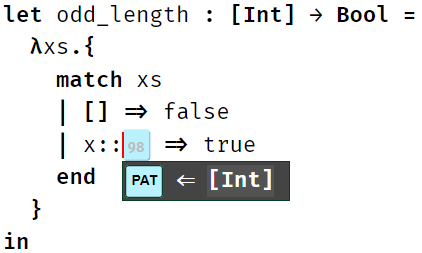
\includegraphics[scale=0.5]{imgs/maybe_exhaustive.png}
}
\hfill
  \subfloat[Must not be exhaustive.\label{fig:not-exhautive}]{
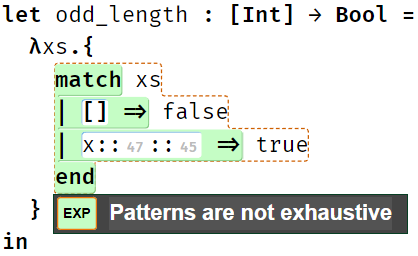
\includegraphics[scale=0.5]{imgs/not_exhaustive.png}
}
  \caption{Exhaustiveness Checking in Incomplete Match Expressions}
  \label{fig:exhaustiveness}
\end{figure}

First we will build the intuition for exhaustiveness checking when there are holes in the patterns of a match expression. When there are holes, we consider if there is a way that the holes could be filled such that the match expression could be exhaustive. If there is, we say that the match expression may or may not be exhaustive. If there is no such way to fill the holes, then the expression must not be exhaustive. Let us look at \autoref{fig:exhaustiveness} for an example using our \texttt{has\_odd\_length} function. We see in \autoref{fig:may-exhaustive} that the pattern of the second match expression contains a hole. This hole could be filled in such that the case is exhaustive, for example using \texttt{xs}. This would have the first branch match empty lists and the second branch match all non-empty lists, making the branches exhaustive. However, the hole in the pattern of the second branch could also be filled in such a way that the branches are not exhaustive, for example using \texttt{y::xs}. In this situation, the second branch would now only match lists that have at least two elements, leaving lists with only one element unmatched. Therefore, we see that this hole filling results in a match with non-exhaustive branches. In our implementation in Hazel, no warnings are shown since the match expression is not yet known to be not exhaustive. It is also possible for a match expression with pattern holes to be not exhaustive. We see in \autoref{fig:not-exhautive} that again the pattern of the match expression contains a hole. However, there is no way to fill in this hole such that the branches are exhaustive. Therefore, Hazel displays a warning message to the programmer.

\begin{figure}[h]
  \centering
    \subfloat[May or may not be redundant. \label{fig:may-redundant}]{
    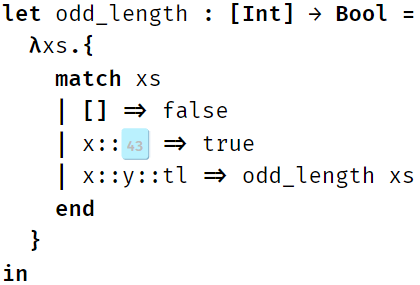
\includegraphics[scale=0.5]{imgs/maybe_redundant.png}
    } 
    \hfill
  \subfloat[Must be redundant. \label{fig:must-redundant}]{
  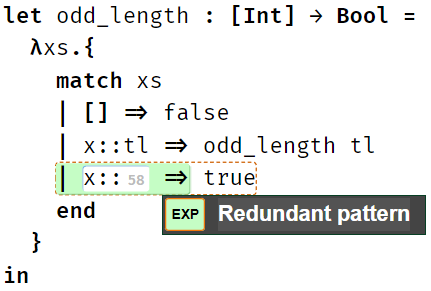
\includegraphics[scale=0.5]{imgs/redundant.png}
  }%
  \caption{Redundancy Checking in Incomplete Match Expressions}
  \label{fig:redundancy}
\end{figure}

Next, let us discuss redundancy checking when pattern holes are present. Similar to exhaustiveness checking, we consider if there is a way that the holes could be filled such that the match expression might not be redundant. If there is, we say that the match expression may or may not be redundant. If there is no such way to fill the holes, then the expression must be redundant. Let us consider the example shown in \autoref{fig:redundancy}. In \autoref{fig:may-redundant}, we see that there is a hole in the second branch of the match expression. It is possible to fill in this hole in a way that would not make the branches redundant, such as the empty list pattern, \texttt{[]}. However, it is also possible that the hole could be filled in a way that causes a redundancy, such as the pattern \texttt{y::xs}. This filling would make the third branch redundant since there is no expression that would match the third that would not first match with the second. Now let us look at \autoref{fig:must-redundant}. Here we see a situation where there is a hole in the pattern for the third branch of the match expression. However, there is no way to fill the hole such that this third branch would not be redundant. This is because the first and second branches will match all empty and non-empty lists, meaning that no expression would be matched by the third branch that would not already have been matched in prior branches. Thus we can see that this third rule must be redundant, and Hazel shows a warning on the redundant rule.

\begin{figure}[h]
\centering
\subfloat[Pattern matching with expression  holes.\label{fig:exp-hole}]{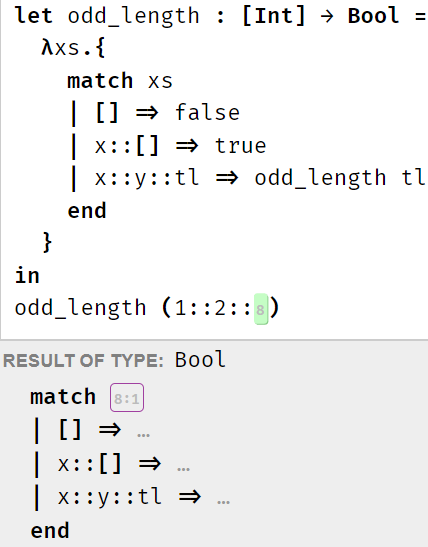
\includegraphics[scale=0.47]{imgs/pat_match_exp_holes.png}}
\hfill
\subfloat[Pattern matching with pattern holes.\label{fig:pat-hole}]{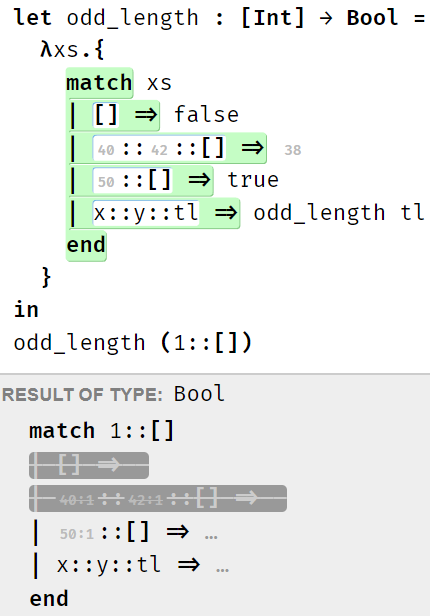
\includegraphics[scale=0.47]{imgs/pat_match_pat_holes.png}}
  \caption{Pattern Matching with Expression Holes}
  \label{fig:evaluation-ex}
\end{figure}

We now move to evaluating case expressions in the presence of pattern and expression holes. We first look at the situation where there are expression holes. We see in \autoref{fig:exp-hole} that the argument to \texttt{has\_odd\_length} has a hole. During evaluation, Hazel checks which pattern matches this expression. We can determine that the first branch does not match since regardless of how the expression hole is filled, the list is not empty. Similarly, we can also determine that the second branch does not match because regardless of how the expression hole is filled, the list is at least of length two. When checking the third branch, we see that we have a pattern that matches a list of at least two elements. As just stated, our list with a hole will have at least two elements regardless of how that hole is filled. Thus, we can take that branch, binding \texttt{xs} to hole \todo{fill in with ending hole number} (hole number are shown as light grey text inside the hole in the Hazel UI). The expression is then evaluated, calling \texttt{has\_odd\_length} again, this time using hole \todo{fill in with ending hole number}. When we evaluate to the case again, we cannot determine which branch to take since the empty hole could match (but also may not) the first rule. Therefore, our evaluation stops. Hazel indicates which branch we stopped on by greying out all previous branches, as can be seen on the bottom of \autoref{fig:exp-hole}.

Next we look at the situation where there are pattern holes during evaluation. We see in \autoref{fig:pat-hole} that we have holes in the patterns of the match expression. We evaluate down to the match expression, branching on \texttt{1::[]}. This does not match the pattern of the first branch, so we move to the second. While the pattern of the second branch has a hole, we are still able to determine that this branch does not match. We can do this because there is no way to fill in hole \todo{fill in with ending hole number} such that that pattern will match a list with two elements. Hazel uses hole based filling, so the only patterns that can fill in the hole have to be for the head of the list, and the head of a list is only one element. We therefore move to the third branch. Here our evaluation stops since in this scenario of a pattern hole, we cannot determine if the expression we are branching on will match this pattern. Therefore, our evaluation stops on the third branch as indicated in the Hazel UI.
